\documentclass[aspectratio=169,xcolor={dvipsnames}]{beamer}
\usepackage[utf8]{inputenc}
\usepackage{graphicx}
\usepackage[turkish]{babel}
\usepackage{amsmath}
\usepackage{amssymb}
\usepackage{booktabs}
\usepackage{tikz}
\usepackage{hyperref}
\usepackage{textcomp} % Derece işareti gibi semboller için eklendi
\usepackage{amsmath}
\usepackage{kvsetkeys}
\let\setkeys\kvsetkeys
\usepackage[utf8]{inputenc}
\usepackage[T1]{fontenc}
\usepackage[turkish]{babel}
\usepackage{rotating}
\usepackage{listings}
\usepackage{xcolor}
\usepackage{tikz}

% Tema seçimi
\usetheme{Madrid}
\usecolortheme{seahorse}



\usebackgroundtemplate{
  \centering
  \tikz\node[opacity=0.1] { % <-- Görüntüyü bir TikZ "node" içine alıyoruz
    
\includegraphics[width=\paperwidth,
                     height=\paperheight]
                    {images/logo.png}
  }; % <-- TikZ komutunu kapatıyoruz
}

% \addtobeamertemplate{block begin}{\pgfsetfillopacity{0.5}}{\pgfsetfillopacity{1}}
% \addtobeamertemplate{block alerted begin}{\pgfsetfillopacity{0.5}}{\pgfsetfillopacity{1}}
% \addtobeamertemplate{block example begin}{\pgfsetfillopacity{0.5}}{\pgfsetfillopacity{1}}







% Başlık bilgileri
\title[Proje No: 3251897]{\textbf{QuatMark}: Dijital İçerik Sahteciliğinin Önlenmesi, Kimlik Doğrulama ve Sızıntı Tespiti için Kriptografi Katmanlı Damgalama Sisteminin Geliştirilmesi}
\subtitle{
\includegraphics[height=2.9ex]{images/pngegg.png} 1501 TÜBİTAK Sanayi AR-GE Projeleri Destekleme Programı}
\author{ QuatVision Yazılım Teknoloji San. Tic. A.Ş.}
%\institute{Proje No: 3251897}


\begin{document}

% Başlık sayfası
\begin{frame}
\titlepage
\end{frame}

% İçindekiler
\begin{frame}{İçindekiler}

\tableofcontents
\end{frame}

% Bölüm 1: Proje Tanıtımı
\section{Proje Tanıtımı}

\begin{frame}{Proje Özeti}

\begin{block}{Proje Adı}
\textbf{QuatMark}: Dijital İçerik Sahteciliğinin Önlenmesi, Kimlik Doğrulama ve Sızıntı Tespiti için Kriptografi Katmanlı Damgalama Sisteminin Geliştirilmesi
\end{block}

\begin{itemize}
\item \textbf{Proje Numarası:} 3251897
\item \textbf{Kuruluş:} QuatVision Yazılım Teknoloji San. Tic. A.Ş.
\item \textbf{Proje Süresi:} 18 ay 
\item \textbf{Teknoloji Grubu:} Bilişim Teknolojileri
\item \textbf{THS Başlangıç:} 3 $\rightarrow$ \textbf{THS Hedef:} 7
\end{itemize}
\end{frame}

\begin{frame}{Kuruluş Tanıtımı}
\begin{block}{QuatVision Hakkında}
QuatVision, bilgisayar görüşü ve dijital veri güvenliği alanlarına yoğunlaşmış bir Ar-Ge şirketidir.
\end{block}

\textbf{Öz Yetkinlikler:}
\begin{itemize}
\item Yüksek matematik 
\item Görüntü işleme ve derin öğrenme algoritmaları
\item Yapay zeka tabanlı görsel denetim sistemleri
\item Dijital damgalama teknolojileri
\end{itemize}

\textbf{Vizyon:} Dijital içeriklerin güvenliği, kimlik doğrulaması ve izlenebilirliği konusunda lider bir rol oynamak
\end{frame}


% Bölüm 2: Projenin Amacı
\section{Projenin Amacı ve Hedefleri}



\begin{frame}{Bilgi Güvenliği}
\begin{block}{Tanım}
Dijital teknolojilerin hızla gelişmesiyle birlikte, internet üzerinden paylaşılan verilerin güvenliği giderek daha önemli hale gelmiştir. Özellikle kişisel verilerin korunması, fikri mülkiyet haklarının güvenliği ve dijital içeriklere yönelik sahteciliğe karşı alınacak önlemler günümüzde büyük bir öncelik taşımaktadır. Bu bağlamda, bilgi güvenliği teknolojileri, dijital verilerin bütünlüğünü ve gizliliğini sağlamada kritik bir rol oynamaktadır. 
\end{block}


\begin{figure}[h]
    \centering
    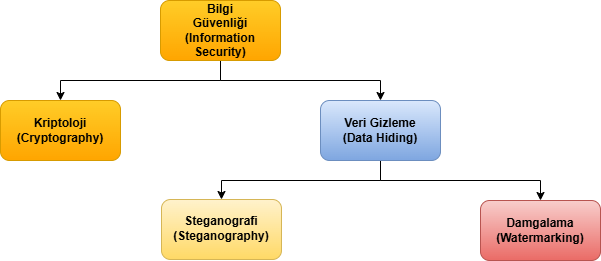
\includegraphics[scale=0.4]{images/data_hiding.png}    
    \label{fig:grafik}
\end{figure}
\end{frame}



\begin{frame}{Bilgi Güvenliği}
\begin{block}{Kriptoloji}
Kriptoloji, verilerin şifrelenmesi ve kodlanması yoluyla, yalnızca yetkili erişimin sağlanması amacıyla kullanılan yöntemleri içerir.  
\end{block}
\begin{block}{Veri Gizleme}
Veri gizleme ise verinin yapısına veya taşıyıcı medyaya entegre edilen ek bilgilerin, yalnızca yetkili kullanıcılar tarafından tespit edilip okunabilmesini sağlayacak biçimde saklanması süreci olarak tanımlanır.  
\end{block}
\textcolor{red}{Veri gizleme işlemi, kriptoloji yöntemleriyle de gerçekleştirilebilir. Ancak, gizlenecek verinin şifrelenmiş ve erişilebilir olması, saldırganların bu verilere yönelik ilgisini artırmakta ve bu durum güvenlik açısından ilave riskler doğurmaktadır.}
\end{frame}




% --- YENİ EKLENEN SLAYT 1 ---
\begin{frame}{Watermarking (Dijital Damgalama) Nedir?}
\begin{block}{Tanım}
Dijital damgalama (watermarking), bir dijital veriye (görüntü, ses, video, metin) gözle görülür veya görünmez bir bilgi (imza, logo, kimlik kodu) ekleme işlemidir.
\end{block}


\begin{figure}[h]
    \centering
    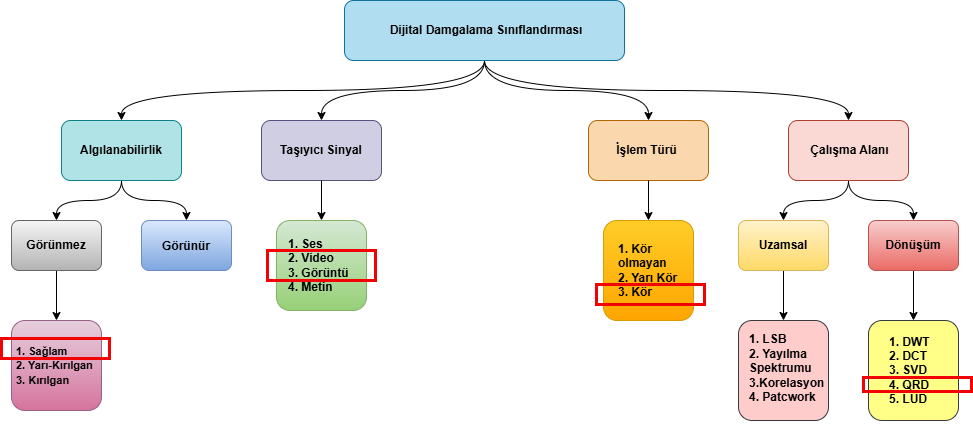
\includegraphics[scale=0.36]{images/siniflandirma.png}    
    \label{fig:grafik}
\end{figure}


\end{frame}

% --- YENİ EKLENEN SLAYT 2 ---
\begin{frame}{Neden Günümüzde İhtiyaç Duyuluyor?}
\begin{alertblock}{Artan Dijital Tehditler}
Dijital içeriklerin kopyalanması, değiştirilmesi ve izinsiz dağıtılması her zamankinden daha kolay hale gelmiştir.
\end{alertblock}

\textbf{Karşılaşılan Temel Sorunlar:}
\begin{itemize}
\item \textbf{Dijital Sahtecilik (Deepfake):} Yapay zeka ile üretilen sahte içerikler (video, ses, görüntü) güveni sarsmaktadır.
\item \textbf{Veri Sızıntıları:} Kurumsal veya askeri nitelikteki gizli belgelerin ve görsellerin kim tarafından sızdırıldığını bilme ihtiyacı artmıştır.
\item \textbf{Telif Hakkı İhlalleri:} Fotoğraf, video ve dijital sanat eserlerinin izinsiz kopyalanması, içerik üreticilerini mağdur etmektedir.
\item \textbf{Bütünlük Kaybı:} Bir medyanın (örn. adli delil, tıbbi görüntü) orijinal ve tahrif edilmemiş olduğunu kanıtlama zorunluluğu vardır.
\end{itemize}
\end{frame}

% --- YENİ EKLENEN SLAYT 3 ---
\begin{frame}{Kullanım Alanları ve Pazar Potansiyeli}
\begin{columns}
\column{0.55\textwidth}
\begin{block}{Yaygın Kullanım Alanları}
\tiny
\begin{itemize}
\item \textbf{Askeri Uygulamalar:} Gizli belgelerin ve stratejik verilerin orijinalliğini koruma.
\item \textbf{Telif Hakkı Koruma:} İçerik sahipliğini belirginleştirerek izinsiz kopyalamayı engelleme.
\item \textbf{Dijital Adli Tıp:} Manipülasyon izlerini takip için delil kaynağını doğrulama.
\item \textbf{Uzaktan Eğitim:} Ders materyallerinin veya sınav içeriklerinin bütünlüğünü koruma.
\item \textbf{Akıllı Sağlık:} Hasta verilerinin gizliliği, sahteciliği önleme.
\item \textbf{Güvenli E-Oylama:} Oy pusulalarını doğrulayarak seçim güvenliğini artırma.
\item \textbf{Lisans Güvenliği:} Yazılım/medya korsanlığını önleme.
\item \textbf{Yayın İzleme:} İçeriklerin platform takibi.
\end{itemize}
\end{block}
\column{0.45\textwidth}
\begin{alertblock}{Pazar Potansiyeli (Grand View Research)}
Damgalama teknolojisi, Avrupa ve Türkiye pazarlarında niş ve yüksek potansiyelli bir alandır.
\vspace{0.3cm}
\textbf{Küresel Pazar Büyüklüğü:}
\begin{itemize}
\item \textbf{2024:} 1.45 Milyar USD
\item \textbf{2033 (Tahmin):} 3.80 Milyar USD
\item \textbf{Yıllık Büyüme (CAGR):} \%11.4 (2025-2033)
\end{itemize}
\end{alertblock}
\end{columns}
\end{frame}


% --- DEĞİŞTİRİLEN SLAYT ---
% Bu slayt artık 3 hizmet için bir giriş niteliğinde
\begin{frame}{Projenin Temel Amacı}
\begin{alertblock}{Ana Hedef}
Eliptik kuaterniyon (4-boyutlu hiperkompleks sayı sistemi) tabanlı kaotik kriptografi katmanlı damga yerleştirme yöntemi geliştirmek.
\end{alertblock}

\textbf{Projenin Çıktısı Olan Hizmetler:}
\begin{itemize}
\item Proje, dijital güvenliğin üç temel sorununa odaklanan bir hizmet paketi sunacaktır:
\item[1.] Veri Sızıntılarını Önleme ve Tespit
\item[2.] İçerik Kimlik Doğrulaması
\item[3.] Fikri Mülkiyet Haklarını Koruma
\item [-] \textcolor{red}{Yayın İzleme (Projenin bir sonraki aşamasında)} 
\item[-] \textcolor{red}{Ses ve metin belgelerine damgalama uygulamaları(Projenin bir sonraki aşamasında)}
\item [-] \textcolor{red}{Fiziksel ürünlere dair damgalama uygulamaları(Projenin bir sonraki aşamasında)}
\end{itemize}
% \begin{block}{Yaklaşım}
% Bu üç hizmet, geliştirilecek olan eliptik kuaterniyon tabanlı sağlam ve kör  damgalama algortiması üzerinden sağlanacaktır.
% \end{block}
\end{frame}


% --- HİZMET 1 İÇİN YENİ SLAYT ---
\begin{frame}{Hizmet 1: Veri Sızıntılarını Önleme ve Tespit}

\begin{block}{Sızıntı Tespit}
Hassas bir belge veya askeri bir görsel birden fazla departmanla/kişiyle paylaşıldığında belgenin güvenliği için:
\end{block}
\textbf{QuatMark Çözümü:}
\begin{itemize}
\item Her bir kopyaya, alıcıya özel, görünmez bir \textbf{dijital parmak izi}  eklenir.
\item İçerik yetkisiz bir yerde yayınlanırsa, sızan belgedeki damga okunur.
\item Sızıntının \textbf{hangi kullanıcıdan} kaynaklandığı tespit edilir.
\item İçeriden gelen tehditlere karşı en güçlü caydırıcılığı sağlar.
\end{itemize}


\end{frame}

% --- HİZMET 2 İÇİN YENİ SLAYT ---
\begin{frame}{Hizmet 2: İçerik Kimlik Doğrulama (Bütünlük)}

\begin{block}{Kimlik Doğrulama}
Özellikle yapay zeka (Deepfake) çağında, bir görüntünün veya belgenin orijinal mi yoksa tahrif edilmiş mi olduğunu anlamak kritiktir.
\end{block}
\textbf{QuatMark Çözümü:}
\begin{itemize}
\item Orijinal içeriğe gömülen damga, bir \textbf{dijital mühür} görevi görür.
\item \textbf{Doğrulama:} Damga okunabiliyorsa içerik \textbf{orijinaldir} ve değiştirilmemiştir.
\item Adli bilişim, tıbbi görüntüler ve haber ajansları için hayati önem taşır.
\end{itemize}


\end{frame}

% --- HİZMET 3 İÇİN YENİ SLAYT ---
\begin{frame}{Hizmet 3: Fikri Mülkiyet Haklarını Koruma}

\begin{block}{Telif Hakkı}
Bir fotoğrafçı, dijital sanatçı veya içerik üreticisi, eserlerinin internette izinsiz kopyalanmasından ve "çalıntı" olarak kullanılmasından endişe duymaktadır.
\end{block}
\textbf{QuatMark Çözümü:}
\begin{itemize}
\item Eserin içine, sahibinin kimlik bilgilerini içeren görünmez bir damga yerleştirilir.
\item Eser internette izinsiz kullanılırsa, damga çıkarılarak eserin \textbf{gerçek sahibi} kanıtlanabilir.
\item Dijital korsanlığa karşı caydırıcılık sağlar.
\item Olası telif hakkı davalarında \textbf{güçlü yasal kanıt} niteliği taşır.
\end{itemize}

\end{frame}
% --- DEĞİŞİKLİK BURADA BİTİYOR ---





% --- Slayt 1: Görünmez Damgalama ---
\begin{frame}{Görünmez Damgalama}

\begin{block}{Görünmez Damgalama}

        Bu yöntemler, yasal delil niteliği sunma ve manipülasyona karşı yüksek dayanıklılık gibi avantajlara sahiptir.

\end{block}

    \begin{block}{Temel Dezavantajlar}
        \begin{itemize}
            \item \textbf{Yüksek Hesaplama Gereksinimi:}
                \begin{itemize}
                    \item Damganın hem görünmezliğini sağlamak hem de manipülasyona karşı yüksek dayanıklılık (robustness) kazandırmak için kullanılan karmaşık algoritmalar, yoğun işlem gücü gerektirir.
                \end{itemize}
            
            
            \item \textbf{Güvenli Anahtar Yönetimi Gerekliliği:}
                \begin{itemize}
                    \item Algoritmanın güvenliği, damga gömme ve çıkarma işlemleri için kullanılan anahtarların gizliliğine ve yönetimine bağlıdır.
                \end{itemize}
        \end{itemize}
    \end{block}
    


\end{frame}

% --- Slayt 2: Kör Damgalama ---
\begin{frame}{Kör Damgalama}
    \begin{block}{Kör Damgalama}
      Kör damgalama özellikle ana dosyanın saklanmasının veya iletilmesinin zor olduğu durumlarda avantaj sağlar. Telif hakkı ihlallerinin tespiti ve içerik sahipliğinin doğrulanması, medya dağıtımı, film, müzik veya dijital yayınlar gibi içeriklerde, ana veriye ulaşılmadan damganın kontrolü imkânı sunar.  
    \end{block}

    \begin{itemize}
        \item \textbf{Doğruluk ve Kesinlik Problemleri:}
        \begin{itemize}
            \item Ana referansın (orijinal görüntünün) olmaması, damganın çıkarımında doğruluk ve kesinlik sorunlarına yol açabilmektedir.
        \end{itemize}
              
        \item \textbf{Dayanıklılık Zafiyetleri:}
        \begin{itemize}
            \item Algoritmanın bazı durumlarda saldırılara karşı dayanıklılığı zayıflayabilmektedir.
        \end{itemize}
        
        
        \item \textbf{Kalite Kaybı Riski:}
        \begin{itemize}
            \item Görüntü işleme işlemleri (örn. sıkıştırma) sırasında damganın zarar görme riski, kalite kaybı olasılığını artırmaktadır.
        \end{itemize}
    \end{itemize}
\end{frame}

% --- Slayt 3: Dönüşüm Uzayı Yöntemleri ---
\begin{frame}{Dönüşüm Uzayı Yöntemleri}

    \begin{block}{Dönüşüm Uzayı}
        Dönüşüm uzayında yapılan damgalama tekniklerinin avantajları arasında saldırılara karşı daha güçlü bir direnç göstermesi ve damga bilgilerinin görüntü kalitesini büyük ölçüde koruyacak şekilde saklanabilmesi yer alır. 
    \end{block}

    \begin{block}{En Önemli Dezavantajlar}
        \begin{itemize}
            \item Yüksek hesaplama maliyeti
            \item Düşük kapasite (gömülebilecek veri miktarının azlığı)
        \end{itemize}
    \end{block}
    
        
    \begin{block}{Kalite Bozulması Riski}
        Dönüştürülmüş bileşenlerin yanlış seçimi ya da uygunsuz güç parametreleri (damga gücü) kullanımı, görüntü kalitesinde gözle görülür bozulmalara neden olabilir.
    \end{block}
    
\end{frame}

% --- Slayt 4: Renkli Görüntü Damgalama (Geleneksel) ---
\begin{frame}{Renkli Görüntü Damgalama Modelleri}
    \begin{block}{Geleneksel Yaklaşım: Kanalların Ayrı İncelenmesi}
        Hem ana görüntünün hem de damga görüntüsünün renk kanallarının (R, G, B) ayrı ayrı incelenmesi neticesinde:
        \begin{itemize}
            \item Renk kanallarının \textbf{korelasyon kaybı}
            \item Damga yerleştirmenin \textbf{asenkronizasyonu}
        \end{itemize}
        gibi dezavantajlar ortaya çıkmaktadır.
    \end{block}
    
    
    \begin{alertblock}{Bu Durumun Sonuçları}
        \begin{itemize}
            \item Modelin doğruluğunun ve verimliliğinin azalması
            \item İşleme süresinin artması
            \item Sonuçların tutarsız olması
        \end{itemize}
    \end{alertblock}
\end{frame}

% --- Slayt 5: Reel Kuaterniyonlar (Zorluklar 1) ---
\begin{frame}{Reel Kuaterniyonlar: Zorluklar}
    \begin{block}{Avantaj}
        Reel kuaterniyonlar, çok kanallı verilerin (renkli görüntülerin) senkron bir şekilde işlenmesinde güçlü bir araçtır; daha az parametreyle daha zengin ilişkiler modelleyebilir.
    \end{block}
    \begin{alertblock}{Dezavantaj: Çarpma İşleminin Değişmeli Olmaması}
        Çarpma işleminin komütatif (değişmeli) olmaması şu sorunları beraberinde getirir:
        \begin{itemize}
            \item Ek hesaplama maliyeti
            \item Algoritmik karmaşıklık
            \item Potansiyel doğruluk sorunları (hata birikimi)
        \end{itemize}
    \end{alertblock}

\end{frame}

% --- Slayt 6: Reel Kuaterniyonlar (Zorluklar 2) ---
\begin{frame}{Reel Kuaterniyonlar: Zorluklar}
    \begin{exampleblock}{Hata Birikimi}
        Komütatif sistemlerde yuvarlama hatasını minimize etmek için işlemlere küçük değerler ile başlanabilir. Ancak reel kuaterniyonlarda çarpma sırası değiştirilemez; bu nedenle hata birikimini azaltacak yeniden sıralama stratejisi uygulanamaz.
    \end{exampleblock}
    \begin{block}{Dezavantaj: Cebirsel Yapının Benzersiz Olmaması}
        Reel kuaterniyonlar cebirinde bir cebirsel yapı benzersiz değildir. Bu durum belirsizliklere yol açar:
        \begin{itemize}
            \item \textbf{Bölme İşlemi:} İki farklı tanım söz konusudur (soldan bölme ve sağdan bölme).

            \item \textbf{Özdeğer/Özvektör:} Tanım çift anlamlıdır (sol özdeğer ve sağ özdeğer).
        \end{itemize}
    \end{block}

    
    \begin{alertblock}{Sonuç}
        Bu durum, reel kuaterniyonları kullanarak denklem çözmede veya gizli damgayı çıkarma işleminde \textbf{belirsizlik} oluşturmakta ve geliştirilen modellerin \textbf{karmaşıklığını} artırmaktadır.
    \end{alertblock}
\end{frame}



















% \begin{frame}{Somut Başarı Ölçütleri}
% \begin{table}
% \centering
% \small
% \begin{tabular}{ll}
% \toprule
% \textbf{Başarı Ölçütü} & \textbf{Hedeflenen Değer} \\
% \midrule
% QR Ayrışımı Hızı (4x4) & $<$ 0.184 ms \\
% QR Ayrışımı Doğruluğu & $<$ 1e-16 \\
% PSNR (Görüntü Kalitesi) & $>$ 40 dB \\
% SSIM (Benzerlik İndeksi) & $>$ 0.98 \\
% NC (Damga Korelasyonu) & $>$ 0.99 \\
% Saldırı Sonrası NC & $>$ 0.98 \\
% API/SaaS Uptime & $>$ 99.9\% \\
% Müşteri Memnuniyeti & $>$ 90\% \\
% \bottomrule
% \end{tabular}
% \end{table}
% \end{frame}

% Bölüm 3: Yenilikçi Yönler
\section{Yenilikçi Yönler ve Teknoloji}

\begin{frame}{Projenin Yenilikçi Yönleri}
\begin{block}{Temel Yenilik}
4-boyutlu \textbf{eliptik kuaterniyonlar} uzayı üzerine inşa edilen damgalama teknolojisi
\end{block}

\textbf{Özgün Teorik Altyapı:}
\begin{itemize}
\item Householder dönüşümü ve QR ayrışımı eliptik kuaterniyonlar cebirinde formüle edilecek
\item Matematiksel kavramlar literatüre doğrudan bilimsel katkı sunacak
\item Patentlenebilir, yenilikçi bir teknoloji
\end{itemize}

\vspace{0.3cm}

\textbf{Teknik Avantajlar:}
\begin{itemize}
\item RGB renk kanallarını bütünleşik olarak işleme
\item Kanallar arası korelasyon kaybının önlenmesi
\item Senkronizasyon hatalarının elimine edilmesi
\item Yüksek saldırı dayanıklılığı
\item Yüksek performans
\end{itemize}
\end{frame}




% Bölüm 4: Teknik Detaylar
\section{Teknik Altyapı ve Metodoloji}

\begin{frame}{Eliptik Kuaterniyon Teorisi}
\begin{block}{Tanım}
Eliptik kuaterniyonlar 4-boyutlu hiperkompleks sayılardır: bir reel ve üç imajiner kısım \[{a_{\left( E \right)}} = {a_{\left( E \right),r}} + {a_{\left( E \right),i}}i + {a_{\left( E \right),j}}j + {a_{\left( E \right),k}}k\] \[\left( {{a_{\left( E \right),r}},{\mkern 1mu} {a_{\left( E \right),i}},{\mkern 1mu} {a_{\left( E \right),j}},{\mkern 1mu} {a_{\left( E \right),k}} \in \mathbf{R},\,\,\,{j^2} = 1,\,\,{i^2} = {k^2} =  p<0,\,,\,\,i,j,k \notin \mathbf{R} } \right).\]
\end{block}

\textbf{Görüntü Temsili:}
\begin{itemize}
\item Her piksel → reel bileşeni sıfır olan eliptik kuaterniyon
\item $m \times n$ piksel görüntü → $m \times n$ boyutlu eliptik kuaterniyon matrisi
\end{itemize}

\begin{figure}[h]
    \centering
    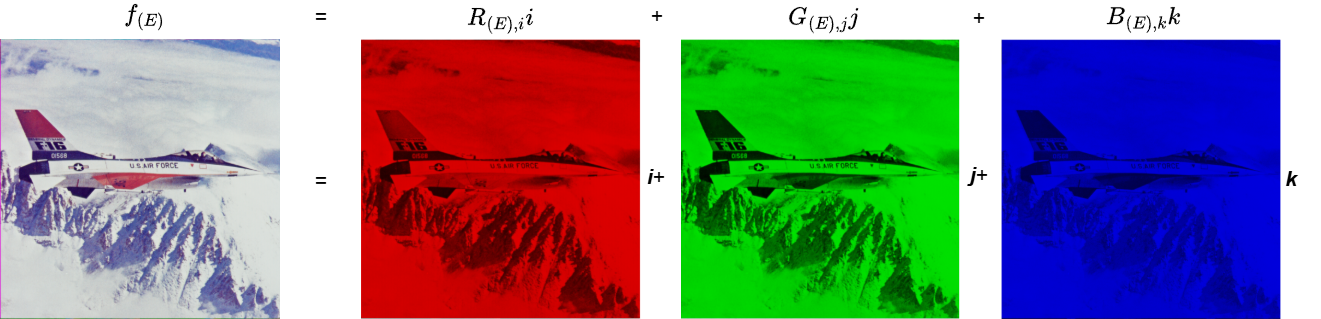
\includegraphics[scale=0.22]{images/airplane_el_rep.png}    
    \label{fig:grafik}
\end{figure}

\end{frame}






\begin{frame}
\begin{block}{$p$ Hiperparametresi}
2023 yılında tamamlanan 121F289 numaralı “Eliptik Kuaterniyon Matris Teorisinin Geliştirilmesi ve Uygulamaları” adlı projesinde elde edilen ${{A}_{\left( E \right)}}{{X}_{\left( E \right)}}={{B}_{\left( E \right)}}$ eliptik kuaterniyonik matris denkleminin en küçük normlu en küçük kareler çözümünün $p$ ve $m$ değerlerine göre hata yüzeyi şekildeki gibidir. Yüzey üstündeki kırmızı noktalar problemin çözümünü optimal yapan $p$ değerlerini göstermektedir. Eliptik kuaterniyonlar cebirindeki $p$ değeri bu uzayda modellenen problemin performansına doğrudan etki etmektedir. Eliptik kuaterniyonlar cebirindeki $p$ değeri önerilen proje kapsamında elde edilecek algoritmanın birimlerinin tamamına da aynı anda etkileyecek hem performans hemde güvenlik parametresi olarak karşımıza çıkmaktadır.
\end{block}


\begin{figure}[h]
    \centering
    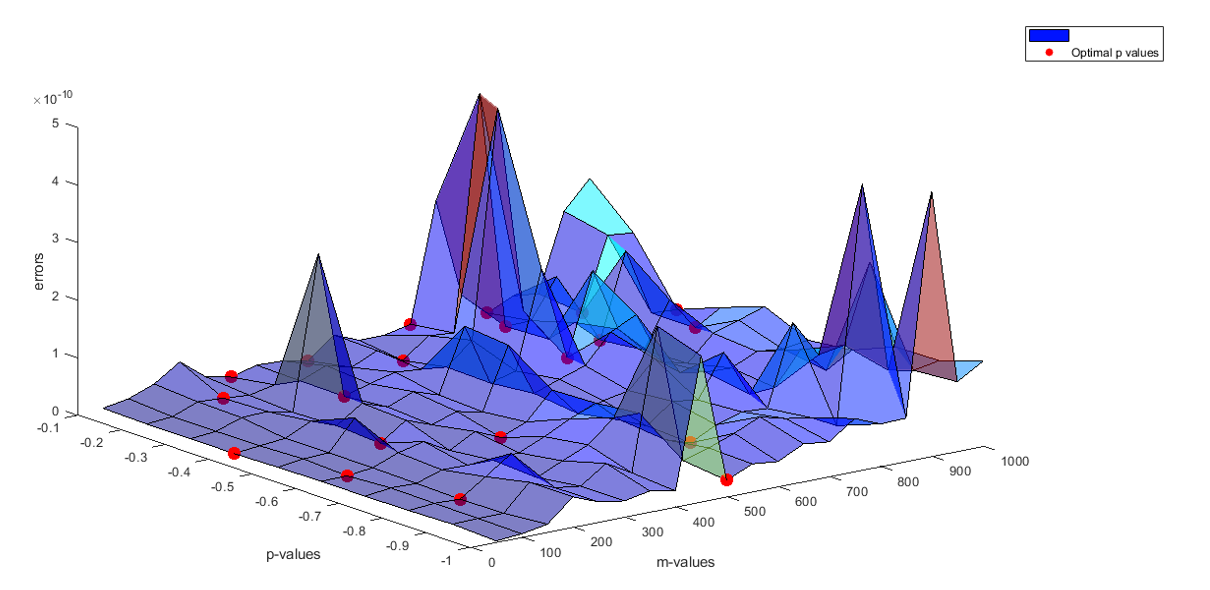
\includegraphics[scale=0.22]{images/hata_yuzeyi.png}    
    \label{fig:grafik}
\end{figure}

\end{frame}



\begin{frame}{Güvenlik Mimarisi}
\textbf{QuatMark Mimarisinin Çok Katmanlı Güvenlik Yapısı:}

\begin{enumerate}
\item \textbf{Arnold Karıştırma:} Damga verisinin uzamsal karıştırması
\item \textbf{Kaotik Şifreleme:} Karıştırılmış damganın şifrelenmesi
\item \textbf{p anahtarı:} İşlemin gerçekleşeceği elliptik uzay
\item \textbf{Hash Tabanlı Konumlandırma:} Pseudo-rastgele blok seçimi
\end{enumerate}

\vspace{0.5cm}

\begin{block}{Avantajlar}
\begin{itemize}
\item Yetkisiz erişime karşı çok katmanlı savunma
\item Her katman ayrı anahtar gerektiriyor
\item Kaba kuvvet saldırılarına karşı direnç
\item Yüksek güvenlik seviyesi
\end{itemize}
\end{block}
\end{frame}



\begin{frame}
    % Slaytın başlığı
    \frametitle{Arnold Karıştırma Algoritması (Arnold'un Kedi Dönüşümü)}

    % --- Tanım Bloğu ---
    \begin{block}{Tanım}
        Arnold'un Dönüşümü, birim kare (genellikle bir görüntü) üzerinde uygulanan \textbf{kaotik} bir dönüşümdür. Görüntüdeki piksellerin yerini belirli bir kurala göre defalarca değiştirerek karıştırmak için kullanılır.
    \end{block}

    % --- Matematiksel Formül Bloğu ---
    \begin{block}{Matematiksel Formül (M x N Görüntü için)}
        $N \times N$ boyutlarındaki bir görüntüde yer alan $(x, y)$ koordinatındaki bir pikselin, bir sonraki iterasyondaki yeni $(x', y')$ konumu şu şekilde hesaplanır:

        % $$...$$ ifadesi, formülün ortalanarak ve "display" modunda yazılmasını sağlar.
        $$
        \begin{pmatrix} x' \\ y' \end{pmatrix} = 
        \begin{pmatrix} 1 & 1 \\ 1 & 2 \end{pmatrix} 
        \begin{pmatrix} x \\ y \end{pmatrix} (mod\, M, mod\, N)
        $$
    \end{block}

\end{frame} % Tek slayt burada biter







% --- Slayt 2: Kaotik Sistemler (Notun üst kısmı) ---
\begin{frame}
  \frametitle{Kaotik Sistemler}
  
  Kaotik sistemler aşağıdaki özelliklere sahip olmaktadır:
  \begin{itemize}
    \item Sözde rasgelelik
    \item Başlangıç değerlerine karşı yüksek hassasiyet
    \item Doğrusal olmama
  \end{itemize}
  
  \vfill % Sayfada dikey boşluk bırakır
  
  \begin{block}{Lojistik Haritası}
    Lojistik haritası:
    
   
    $$ X_{k} = \mu X_{k-1}(1 - X_{k-1}) $$
    
    Burada:
    \begin{itemize}
        \item $X_k \in (0,1)$
        \item $\mu$ (kontrol parametresi) için kaosa geçiş değeri:
        \item $\mu \approx 3.5699456...$
    \end{itemize}
    
    % Notlarda ilk yazılan (muhtemelen hatalı) formül:
    % $$ X_k = \mu(X_k)(X_{k-1}) $$
    
  \end{block}
\end{frame}

% --- Slayt 3: Kaotik Şifreleme Uygulaması (Notun alt kısmı) ---
\begin{frame}
  \frametitle{Kaotik Şifreleme ile Görüntü İşleme}
  
  \begin{block}{Amaç}
    Kaotik şifreleme ile görüntünün istatistiksel saldırılara karşı daha etkili bir şekilde direnmesi sağlanır.
  \end{block}
  
  \vfill
  
  \begin{block}{Adımlar}
    \begin{enumerate}
      \item Damga Görüntüsü (M x N boyutlarında)
      \item M ve N değerleri girdi olarak alınır.
      \item R matrisi oluşturulur.
      \item Bozucu matris ($R_1$) aşağıdaki formülle hesaplanır:
      % Not: "round(1000 R(i,j)) mod 255"
      $$ R_1(i,j) = \text{round}(1000 \cdot R(i,j)) \pmod{255} $$
      
      \item Damga verisi ile Bozucu matris ($R_1$), XOR işlemine tabi tutulur.
    \end{enumerate}
  \end{block}
  
\end{frame}



% --- Slayt 2: Hash Fonksiyonları (Genel Tanım) ---
\begin{frame}
  \frametitle{Hash Fonksiyonları}
  
  \begin{block}{Tanım}
    Bir hash fonksiyonu, herhangi bir veriyi alıp onu sabit boyutlu, benzersiz bir özet dizisine dönüştüren matematiksel bir işlemdir.
  \end{block}
  
  \vfill
  
  \begin{block}{Yaygın Algoritmalar ve Güvenlik Durumları}
    \begin{itemize}
      \item MD5 (128-bit) - \textit{Güvensiz (çakışmalara çok açık).}
      \item SHA-1 (160-bit) - \textit{Güvensiz (çakışma saldırılarına açık).}
      \item SHA-2 (256/512-bit) - \textit{Güvenli, günümüzde endüstri standardı.}
      \item SHA-3 (256/512-bit) - \textit{Güvenli, SHA-2'ye modern ve farklı bir alternatif.}
    \end{itemize}
  \end{block}
  
\end{frame}


\begin{frame}
  \frametitle{Metodoloji: Hash Fonksiyonu Değerlendirmesi}
  
  \begin{block}{Temel Yaklaşım: PRNG Tohumlama}
    Damgalama algoritmamız, host görüntüden hangi blokların seçileceğini belirlemek için bir Sözde Rastgele Sayı Üreteci (PRNG) kullanır.
    \vfill
    Bu PRNG'nin "tohum" (seed) değeri, kullanıcı anahtarına (key) uygulanan bir hash fonksiyonunun çıktısından elde edilir.
    \vfill
  \end{block}
  
  
  \begin{alertblock}{Değerlendirme Stratejisi: Neden MD5 ile Başlıyoruz?}
    \begin{itemize}
        \item \textbf{1. Aşama:} Amacımız, teorik bir zayıflığın (çakışma - collision) pratik olarak damgalama algoritmamızı nasıl etkilediğini görmektir.
        \item \textbf{2. Aşama:} Takip eden analizlerde, aynı anahtar ile MD5, SHA-1, SHA-256 ve SHA-3 çıktılarını kullanarak algoritmanın sağlamlığını (robustness) karşılaştıracağız.
        \item \textbf{Sonuç:} Bu yaklaşım, hash fonksiyonu güvenliğinin, damgalama sisteminin güvenliği üzerindeki \textit{pratik etkisini} ölçmemizi sağlayacaktır.
    \end{itemize}
  \end{alertblock}
  
\end{frame}





% --- Slayt 2: İndeks Seçme Aşamaları (1/2) ---
\begin{frame}
  \frametitle{İndeks Seçme Aşamaları (1/2)}
  
  \begin{block}{Adım 1: Hash Çıktısı}
    Anahtar, hash fonksiyonuna verilir ve $2^n$ (MD5 için $n=5$, SHA 256 için $n=6$) karakterlik bir hash çıktısı alınır.
    \begin{itemize}
      \item Bu çıktı 16'lık (hexadecimal) tabanda üretilir.
    \end{itemize}
  \end{block}
  
  \begin{block}{Adım 2: Tabana Dönüştürme}
    Hash fonksiyonunun ürettiği $2^n$ karakterlik 16'lık tabanda yazılmış sayı, 10'luk (decimal) tabana çevrilir.
  \end{block}
  
  \begin{block}{Adım 3: Tohum (Seed) Oluşturma}
    Bu 10'luk tabandaki sayı, sözde-rastgele sayı üretecinin tohumu (seed) olarak kullanılır.
  \end{block}
  
\end{frame}

% --- Slayt 3: İndeks Seçme Aşamaları (2/2) ---
\begin{frame}
  \frametitle{İndeks Seçme Aşamaları (2/2)}
  
  \begin{block}{Adım 4: Rastgele Blok Seçimi Algoritması}
    N adet rasgele blok seçilir.
    
    \vfill
    
    % \texttt{} komutu, kod benzeri yazılar için sabit genişlikli bir font sağlar.
    % \\ komutu satırı sonlandırır.
    % \hspace{1cm} komutu, döngü içi için girinti sağlar.
    
    \textbf{Sözde-Kod (Pseudo-code):}
    
    \texttt{current\_val = hash\_val (tohum)} \\
    \texttt{selected\_blocks = set()} \\
    \texttt{while (döngü devam ettikçe)} \\
    \hspace{1cm} \texttt{idx = current\_val \% N} \\
    \hspace{1cm} \texttt{selected\_blocks.append(block[idx])} \\
    \hspace{1cm} \texttt{current\_val = (current\_val * 1103515245 + 12345) \& 0xFFFFFFFFFFFFFFFF}
    
    \vfill
    (LCG: Linear Congruential Generator / Doğrusal Uyumluluk Üreteci)
    
  \end{block}
  
  
\end{frame}


















\begin{frame}{Damgalama Süreci}
\begin{enumerate}
\item \textbf{Ön İşleme:}
\begin{itemize}
\item Damga verisi Arnold dönüşümü ile karıştırılır
\item Kaotik şifreleme uygulanır
\item 8 bitlik ikili dizilere dönüştürülür
\end{itemize}

\item \textbf{Gömme:}
\begin{itemize}
\item Ana görüntü $4 \times 4$ bloklara ayrılır
\item MD5 ile pseudo-rastgele bloklar seçilir
\item Her bloğa QR ayrışımı uygulanır
\item Damga bitleri $R(1,4)$ elemanına kuantalama ile gömülür
\end{itemize}

\item \textbf{Çıkarma:}
\begin{itemize}
\item Damgalı görüntüden aynı bloklar tespit edilir
\item QR ayrışımı ve ters kuantalama uygulanır
\item Ters Arnold ve kaotik deşifreleme ile orijinal damga elde edilir
\end{itemize}
\end{enumerate}
\end{frame}







\begin{frame}{Damga Gömme Süreci}
\begin{figure}[h]
    \centering
    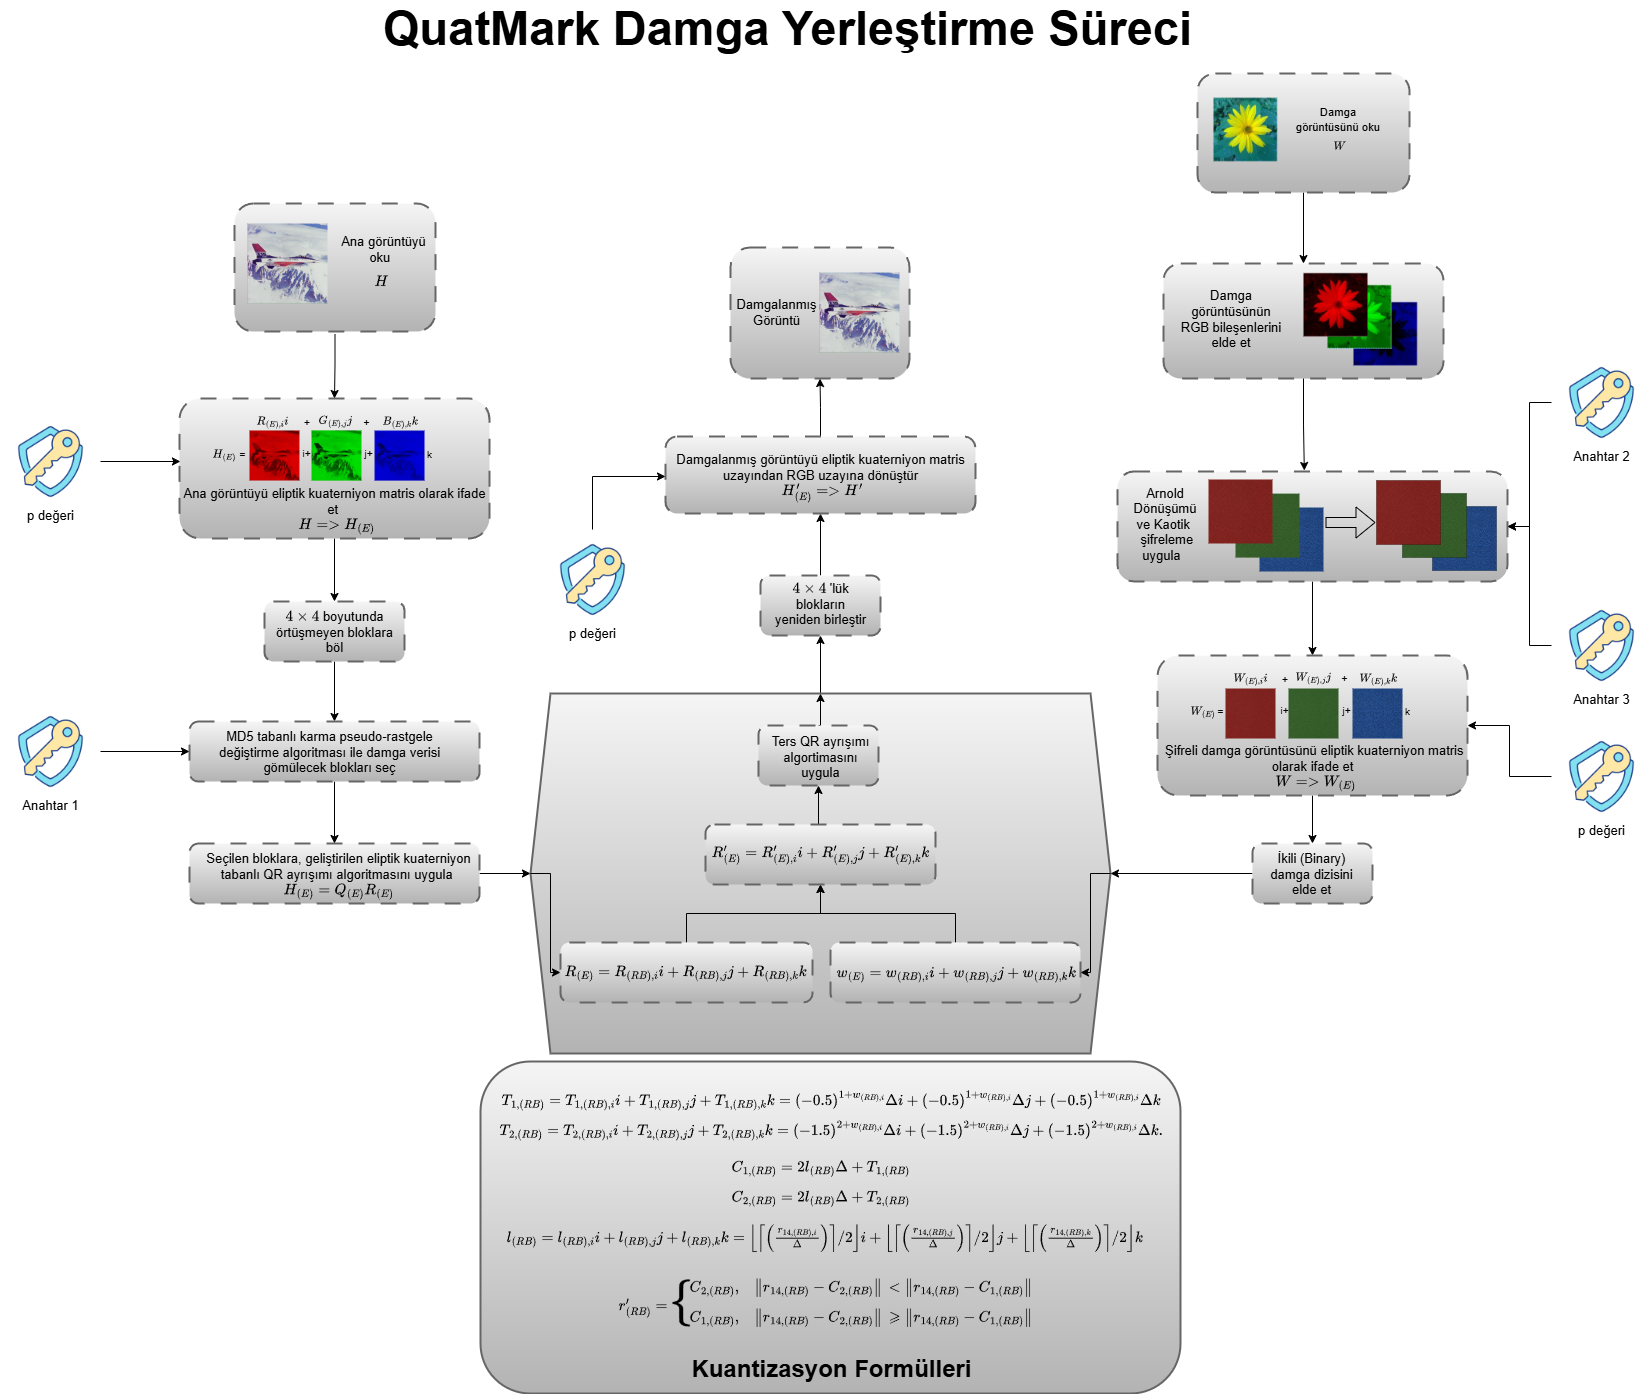
\includegraphics[scale=0.20]{images/GORSEL1.png}    
    \label{fig:grafik}
\end{figure}

\end{frame}



\begin{frame}{Damga Çıkarma Süreci}
\begin{figure}[h]
    \centering
    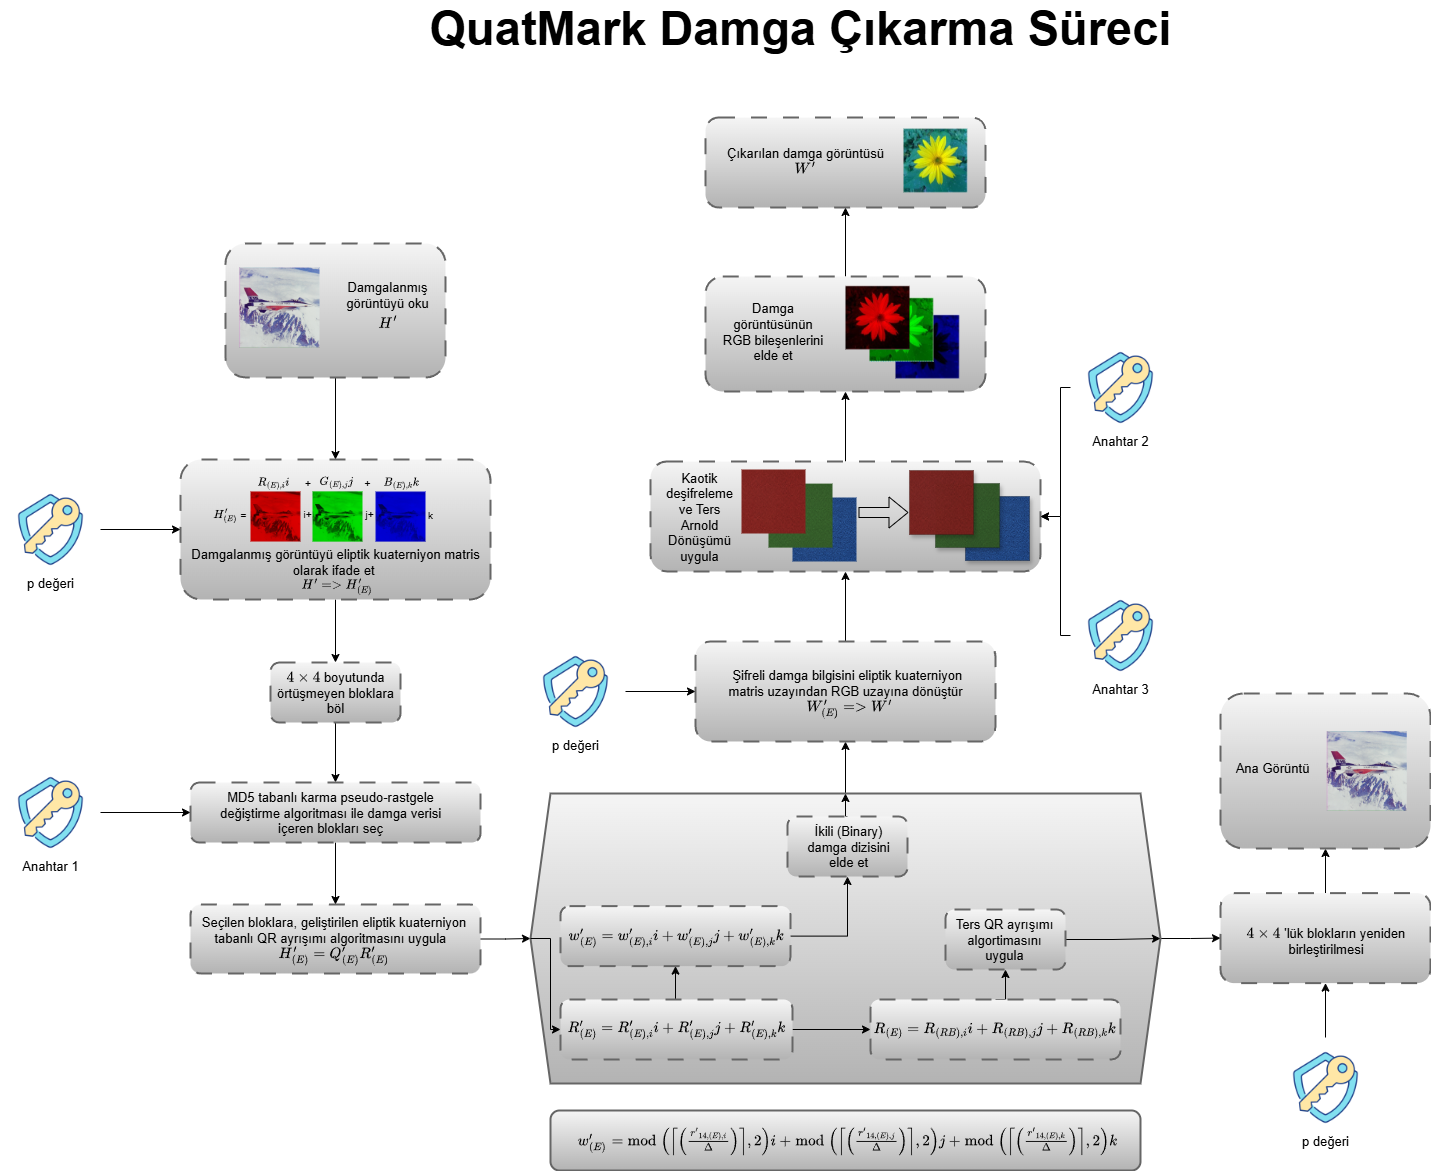
\includegraphics[scale=0.22]{images/GORSEL2.png}    
    \label{fig:grafik}
\end{figure}

\end{frame}





\begin{frame}{Performans Kriterleri}
\textbf{Algılanamazlık (Imperceptibility):}
\begin{itemize}
\item PSNR (Peak Signal-to-Noise Ratio) $>$ 40 dB
\item SSIM (Structural Similarity Index) $>$ 0.98
\item Damgalı görüntü orijinalden ayırt edilemez
\end{itemize}

\vspace{0.3cm}

\textbf{Sağlamlık (Robustness):}
\begin{itemize}
\item Geleneksel saldırılara karşı $NC > 0.98$
\begin{itemize}
\item JPEG sıkıştırma (kalite faktörü $\geq$ 70)
\item Geometrik dönüşümler ($\pm 10$\textdegree~döndürme, $\pm 10\%$ ölçeklendirme)
\item Kırpma (\%80'e kadar), gürültü (SNR $\geq$ 30 dB)
\end{itemize}
\item Derin öğrenme saldırılarına karşı $NC > 0.95$
\end{itemize}
\end{frame}



% Bölüm 5: Uygulama Alanları
\section{Uygulama Alanları ve Hedef Kitle}

\begin{frame}{Hedef Sektörler}
\begin{enumerate}
\item \textbf{Medya ve Yayıncılık:}
\begin{itemize}
\item Haber ajansları, fotoğrafçılar, prodüksiyon şirketleri
\item Telif hakkı koruması ve dijital korsanlığın önlenmesi
\end{itemize}

\item \textbf{Savunma Sanayii:}
\begin{itemize}
\item Askeri teknoloji kuruluşları, istihbarat birimleri
\item Hassas görsel verilerin bütünlük kontrolü
\item Sızıntı tespiti ve kaynak belirleme
\end{itemize}

\item \textbf{Sağlık Bilişimi:}
\begin{itemize}
\item Hastaneler, tıbbi görüntüleme merkezleri
\item Tıbbi görüntülerin orijinallik doğrulaması
\item Hasta verilerinin gizliliği
\end{itemize}

\item \textbf{Adli Bilişim ve Hukuk:}
\begin{itemize}
\item Emniyet birimleri, adli tıp kurumları
\item Dijital delillerin bütünlük doğrulaması
\end{itemize}
\end{enumerate}
\end{frame}

\begin{frame}{Uygulama Senaryoları (Özet)}
    \begin{enumerate} % Manuel 1. 2. 3. yerine otomatik numaralı liste
        \item \textbf{Telif Hakkı Koruması:}
            \begin{itemize}
            \item Dijital içeriğe telif bilgisi gömülür
            \item İzinsiz kullanım tespit edilir
            \item Yasal delil niteliği taşır
            \end{itemize}

        \item \textbf{Kimlik Doğrulama:}
            \begin{itemize}
            \item İçeriğin orijinalliği teyit edilir
            \item Manipülasyon tespit edilir
            \item Güvenilirlik sağlanır
            \end{itemize}

        \item \textbf{Sızıntı Tespiti:}
            \begin{itemize}
            \item Her kopyaya benzersiz damga eklenir
            \item Sızıntı kaynağı kesin olarak belirlenir
            \item İçeriden tehditler önlenir
            \end{itemize}
    \end{enumerate}
\end{frame}

% Bölüm 6: Ürün ve Hizmetler
\section{Ürün Geliştirme ve Ticarileşme}

\begin{frame}{QuatMark Ürün Yapısı}
\begin{columns}
\column{0.5\textwidth}
\begin{block}{SaaS Platform}
\textbf{Web Tabanlı Hizmet}
\begin{itemize}
\item Kullanıcı dostu arayüz
\item Manuel damgalama
\item Abonelik modeli
\item İstatistik ve raporlama
\end{itemize}
\end{block}

\column{0.5\textwidth}
\begin{block}{API Entegrasyonu}
\textbf{Geliştirici Araçları}
\begin{itemize}
\item RESTful API
\item Otomatik damgalama
\item Sistem entegrasyonu
\item Ölçeklenebilir altyapı
\end{itemize}
\end{block}
\end{columns}

\vspace{0.5cm}

\textbf{API Endpoints:}
\begin{itemize}
\item \texttt{POST /v1/watermark/embed} - Damga gömme
\item \texttt{POST /v1/watermark/extract} - Damga çıkarma
\item \texttt{GET /v1/account/status} - Hesap durumu
\end{itemize}
\end{frame}

\begin{frame}{İş Modeli ve Gelir Kaynakları}
\textbf{1. Abonelik Tabanlı Gelirler (SaaS):}
\begin{itemize}
\item Bireysel ve kurumsal paketler
\item Aylık/yıllık abonelik planları
\item Kullanım sınırlarına göre fiyatlandırma
\end{itemize}

\textbf{2. Kurumsal Lisanslama (API):}
\begin{itemize}
\item Doğrudan API lisans satışı
\item Kotalı abonelik modeli
\item Kurumsal müşterilere özel çözümler
\end{itemize}

\textbf{3. Danışmanlık ve Destek:}
\begin{itemize}
\item Teknik entegrasyon desteği
\item Özelleştirilmiş çözümler
\item Eğitim ve dokümantasyon
\end{itemize}
\end{frame}

\begin{frame}{Pazar Analizi}
\begin{block}{Küresel Pazar}
\begin{itemize}
\item 2024: 1.45 milyar USD
\item 2033 Beklenti: 3.80 milyar USD
\item Yıllık Büyüme: \%11+
\end{itemize}
\end{block}

\textbf{Pazar Payı Hedefleri:}
\begin{table}
\centering
\begin{tabular}{lcc}
\toprule
\textbf{Yıl} & \textbf{Hedef Pay} & \textbf{Strateji} \\
\midrule
1. Yıl & \%2-3 & Referans müşteriler \\
3. Yıl & \%8-10 & Pazar penetrasyonu \\
5. Yıl & \%15-20 & Pazar liderliği \\
\bottomrule
\end{tabular}
\end{table}
\end{frame}

% Bölüm 7: İş Planı
\section{Proje İş Planı}

\begin{frame}{İş Paketleri - Genel Bakış}
\begin{columns}[t] % Sütunları dikeyde üstten hizalar

% --- SOL SÜTUN ---
\column{0.5\textwidth}
\textbf{İş Paketi 1:} Teorik Altyapı
\begin{itemize}
\item Householder dönüşümü ve QR ayrışımı teorilerinin geliştirilmesi
\item RBquaternion.py Python modülünün oluşturulması
\end{itemize}

\vspace{1cm} % İki paket arasına dikey boşluk ekler

\textbf{İş Paketi 2:} Damgalama Modeli
\begin{itemize}
\item Dijital damgalama algoritmasının geliştirilmesi
\item Performans testleri ve saldırılara karşı dayanıklılık analizleri
\end{itemize}

% --- SAĞ SÜTUN ---
\column{0.5\textwidth}
\textbf{İş Paketi 3:} Ürünleştirme
\begin{itemize}
\item API ve SaaS platformlarının geliştirilmesi
\item Bulut altyapısının kurulması
\end{itemize}

\vspace{1cm} % İki paket arasına dikey boşluk ekler

\textbf{İş Paketi 4:} Pazara Sunma
\begin{itemize}
\item Pazarlama stratejisi ve lansmanı
\item Sürdürülebilirlik faaliyetleri
\end{itemize}

\end{columns}
\end{frame}

\begin{frame}{Proje Ekibi}
\begin{columns}[t] % Sütunları dikeyde üstten hizala

% --- SOL SÜTUN (YÖNETİCİ KADRO) ---
\column{0.5\textwidth}
\textbf{Ana Personel:}
\begin{itemize}
\item \textbf{Doç. Dr. Hidayet Hüda Kösal}
    \begin{itemize}
    \item Teknoloji Direktörü, Ar-Ge Sorumlusu
    \item Teorik altyapı ve bilimsel koordinasyon
    \end{itemize}

\vspace{0.5cm} % Kişiler arası boşluk

\item \textbf{Samet Ergin}
    \begin{itemize}
    \item Genel Müdür (CEO), Operasyon Direktörü
    \item Yazılım geliştirme ve operasyonel yönetim
    \end{itemize}
\end{itemize}

% --- SAĞ SÜTUN (EKİP VE TOPLAM) ---
\column{0.5\textwidth}
\begin{itemize}
\item \textbf{Ar-Ge Mühendisleri (2)}
    \begin{itemize}
    \item Algoritma geliştirme ve test
    \end{itemize}

\vspace{0.5cm} % Kişiler arası boşluk

\item \textbf{Araştırmacı}
    \begin{itemize}
    \item Teorik destek ve analiz
    \end{itemize}
\end{itemize}

\vfill % Kalan dikey boşluğu doldurarak "Toplam"ı aşağı iter

\begin{block}{Toplam Adam-Ay}
\textbf{Toplam:} 53.58 adam-ay
\end{block}

\end{columns}
\end{frame}

% Bölüm 8: Bütçe
\section{Proje Bütçesi}

\begin{frame}{Bütçe Dağılımı}
\begin{table}
\centering
\small
\begin{tabular}{lrr}
\toprule
\textbf{Maliyet Kalemi} & \textbf{Tutar (TL)} & \textbf{Oran} \\
\midrule
Personel Giderleri & 4.847.600 & \%59.57 \\
Yurtiçi Danışmanlık ve Hizmet & 2.790.000 & \%34.29 \\
Alet/Teçhizat/Yazılım & 250.000 & \%3.07 \\
Yurtiçi Ar-Ge ve Test & 150.000 & \%1.84 \\
Seyahat Giderleri & 100.000 & \%1.23 \\
\midrule
\textbf{TOPLAM} & \textbf{8.137.600} & \textbf{\%100} \\
\bottomrule
\end{tabular}
\end{table}

\vspace{0.3cm}

\end{frame}

% Bölüm 9: Riskler ve Önlemler
\section{Risk Yönetimi}

\begin{frame}{Potansiyel Riskler ve Önlemler}
\begin{table}
\centering
\tiny
\begin{tabular}{p{4cm}p{4cm}p{4cm}}
\toprule
\textbf{Risk} & \textbf{Önlem} & \textbf{B Planı} \\
\midrule
Performans hedeflerinin karşılanamaması & e1,e2 bazı kullanımı & Farklı temsiller denenmesi \\
MD5 güvenlik zafiyeti & Kaotik şifreleme & SHA-256'ya geçiş \\
Arnold dönüşümü zayıflığı & Çok katmanlı güvenlik & Genelleştirilmiş Arnold \\
Derin öğrenme saldırıları & 4D kompleks yapı & Çifte Arnold karıştırma \\
Saldırılara düşük dayanıklılık & Yeni kuantalama & Reed-Solomon kodları \\
Bütçe yetersizliği & Düzenli takip & Öz kaynaklar \\
\bottomrule
\end{tabular}
\end{table}
\end{frame}

% Bölüm 10: Beklenen Çıktılar
\section{Beklenen Çıktılar ve Etkiler}

\begin{frame}{Proje Çıktıları}
\textbf{Teknolojik Çıktılar:}
\begin{itemize}
\item Eliptik kuaterniyon tabanlı QR ayrışımı teorisi
\item Equaternion.py Python modülü
\item QuatMark damgalama algoritması
\item API ve SaaS platformları
\end{itemize} % <--- HATA DÜZELTİLDİ

\vspace{0.3cm}

\textbf{Bilimsel Çıktılar:}
\begin{itemize}
\item Uluslararası dergilerde yayınlar
\item Patent başvuruları
\item Literatüre özgün katkı
\end{itemize}

\vspace{0.3cm}

\textbf{Ticari Çıktılar:}
\begin{itemize}
\item Ticari ürün (QuatMark)
\item Yerli ve milli teknoloji
\item İhracat potansiyeli
\end{itemize}
\end{frame}

\begin{frame}{Ekonomik ve Ulusal Kazanımlar}
\textbf{Ekonomik Katkılar:}
\begin{itemize}
\item Yerli ve milli dijital damgalama teknolojisi
\item İthal ikamesi
\item Yüksek katma değerli ürün
\item İhracat potansiyeli
\end{itemize}

\vspace{0.3cm}

\textbf{Bilimsel ve Teknolojik İlerleme:}
\begin{itemize}
\item Yeni matematiksel teorilerin geliştirilmesi
\item Veri güvenliği alanında yeni uygulamalar
\item Literatüre özgün katkı
\end{itemize}

\vspace{0.3cm}

\textbf{İnsan Kaynağı Gelişimi:}
\begin{itemize}
\item Nitelikli araştırmacı ve mühendis yetiştirilmesi
\item Disiplinler arası bilgi birikimi
\item Ulusal rekabet gücünün artırılması
\end{itemize} % <--- Düzeltilmiş hali
\end{frame}

\begin{frame}{Öncelikli Alan Uyumu}
\begin{block}{12. Kalkınma Planı Uyumu}
Proje, Bilişim ve İletişim Teknolojileri öncelikli alanı altında konumlanmaktadır.
\end{block}

\textbf{Özel Öncelik:}
\begin{itemize}
\item Savunma sektörü için siber güvenlik çözümleri
\item Veri kaçağını önleme teknolojileri
\item Kod güvenliği ve saldırı tespit sistemleri
\end{itemize}

\vspace{0.3cm}

\textbf{Stratejik Önem:}
\begin{itemize}
\item Kritik teknoloji alanında yerli çözüm
\item Dışa bağımlılığın azaltılması
\item Teknoloji ve ürün geliştirme yetkinliğinin artması
\item Ulusal güvenlik katkısı
\end{itemize}
\end{frame}

% Bölüm 11: Rekabet Avantajı
% \section{Rekabet Avantajı}

% \begin{frame}{Rakip Analizi}
% \begin{table}
% \centering
% \tiny
% \begin{tabular}{lcccc}
% \toprule
% \textbf{Özellik} & \textbf{QuatMark} & \textbf{Digimarc} & \textbf{Imatag} & \textbf{Echomark} \\
% \midrule
% Temel Metod & Eliptik Kuaterniyon & Ticari Sır & Ticari Sır & Ticari Sır \\
% Çalışma Uzayı & 4-Boyutlu & Frekans & Frekans & Biçimsel \\
% Taşıyıcı & Görüntü, Video & Çoklu & Çoklu & Metin, PDF \\
% Güvenlik & Çok Katmanlı & Yedekli & Ticari Sır & Çift Katman \\
% Hizmetler & 3 Ana Hizmet & 3 Ana Hizmet & Ticari Sır & Sızıntı Tespiti \\
% \midrule
% \multicolumn{5}{l}{\textbf{Avantaj:} Açık ve bilimsel olarak kanıtlanmış yöntem} \\
% \multicolumn{5}{l}{\textbf{Avantaj:} Yerli ve milli teknoloji} \\
% \multicolumn{5}{l}{\textbf{Avantaj:} Yüksek performans ve dayanıklılık} \\
% \bottomrule
% \end{tabular}
% \end{table}
% \end{frame}

\begin{frame}{Rekabetçi Üstünlükler}
\begin{enumerate}
\item \textbf{Bilimsel Üstünlük:}
\begin{itemize}
\item Akademik olarak kanıtlanmış yöntem
\item Şeffaf ve doğrulanabilir teknoloji
\item Yüksek performans metrikleri
\end{itemize}

\item \textbf{Stratejik Avantaj:}
\begin{itemize}
\item Yerli ve milli çözüm
\item Dışa bağımlılığın azaltılması
\item Ulusal güvenlik önceliği
\end{itemize}

\item \textbf{Teknik Avantaj:}
\begin{itemize}
\item 4-boyutlu bütünleşik işleme
\item Korelasyon koruması
\item Üstün saldırı dayanıklılığı
\end{itemize}

\item \textbf{Ticari Avantaj:}
\begin{itemize}
\item Esnek iş modeli (SaaS + API)
\item Ölçeklenebilir altyapı
\item Rekabetçi fiyatlandırma
\end{itemize}
\end{enumerate}
\end{frame}

% Bölüm 12: Sonuç
\section{Sonuç ve Vizyon}

\begin{frame}{Proje Sonuçları - Özet}
\begin{block}{Teknolojik İnovasyon}
Eliptik kuaterniyon tabanlı, yüksek performanslı ve dayanıklı bir dijital damgalama sistemi
\end{block}

\textbf{Ana Başarı Kriterleri:}
\begin{itemize}
\item Teorik altyapının oluşturulması
\item Yenilikçi algoritmanın geliştirilmesi
\item Ticari ürünün pazara sunulması
\item Yerli ve milli teknoloji üretimi
\end{itemize}

\vspace{0.3cm}

\textbf{Beklenen Etkiler:}
\begin{itemize}
\item Dijital güvenlik alanında teknolojik ilerleme
\item Stratejik sektörlerde dışa bağımlılığın azalması
\item Bilimsel literatüre özgün katkı
\item Yüksek katma değerli ürün ve hizmet
\end{itemize}
\end{frame}

\begin{frame}{Gelecek Vizyonu}
\textbf{Kısa Vadeli Hedefler (1-2 Yıl):}
\begin{itemize}
\item Projenin başarıyla tamamlanması
\item QuatMark ürününün lansmanı
\item Referans müşterilerin edinilmesi
\item Patent başvurularının tamamlanması
\end{itemize}

\textbf{Orta Vadeli Hedefler (3-5 Yıl):}
\begin{itemize}
\item Türkiye pazarında lider konum
\item Pazar payının \%15-20'ye çıkarılması
\item Uluslararası pazarlara açılma
\item Ürün portföyünün genişletilmesi
\end{itemize}

\textbf{Uzun Vadeli Vizyon:}
\begin{itemize}
\item Küresel pazarda tanınan marka
\item Dijital güvenlik alanında teknoloji lideri
\item Sürekli inovasyon ve Ar-Ge
\end{itemize}
\end{frame}

\begin{frame}{İletişim Bilgileri}
\begin{center}
\Large{\textbf{QuatVision Yazılım Teknoloji San. Tic. A.Ş.}}


\vspace{1cm}

\textbf{Proje Yürütücüsü:}

Doç. Dr. Hidayet Hüda Kösal

%\vspace{0.5cm}

\textbf{İletişim:}

hhkosal@quatvision.ai

Tel: 0530-9722035

%\vspace{0.5cm}

\textbf{Adres:}

Esentepe Mah. Akademiyolu Sk. No: 10/6 İç Kapı: 138

Esentepe 54050 Serdivan / SAKARYA

\end{center}
\end{frame}

\begin{frame}
\Huge{\textbf{Teşekkürler}}

\vspace{1cm}

\Large{Sorular?}
\end{frame}

\end{document}